% !TeX program = lualatex

% Per https://github.com/matze/mthemem, Fira fonts needs to be installed in the system.
% If fonts do not metter, just use pdflatex instead of lualatex (and also remove luatex85 depnedency below)

\documentclass{beamer}
\usetheme{metropolis}

\usepackage{luatex85}
\usepackage{graphicx}
\usepackage{qrcode}

\usepackage{mathtools}
\mathtoolsset{showonlyrefs}

% https://stackoverflow.com/a/722954/2098471
\usepackage{chngpage}
\newenvironment{widecenter}{\begin{adjustwidth}{-1cm}{-1cm}\begin{center}}{\end{center}\end{adjustwidth}}

\usepackage[absolute,overlay]{textpos}
\setlength{\TPHorizModule}{\paperwidth}
\setlength{\TPVertModule}{\paperheight}

% https://tex.stackexchange.com/a/43005
\newlength{\currentparskip} 
\newenvironment{minipageparskip}[1]{\setlength{\currentparskip}{\parskip}\begin{minipage}{#1}\setlength{\parskip}{\currentparskip}}{\end{minipage}}

\usepackage{multimedia}
\setlength\unitlength{1cm}
\newcommand{\resvideo}[3]{\movie[width=#2cm,height=#3cm,poster,loop]{\framebox(#2,#3){\includegraphics[width=0.375cm]{res/video.png}\texttt{ #1{\footnotesize.mp4}}}}{video/#1.mp4}}

\usepackage{tikz}
\usetikzlibrary{arrows}
\usepackage{pgfplots}

% END OF CONFIGURATION

\title{MAE 259B Group 2 Progress Report}
\date{05/09/2018}
\author{Siyuan Chen, Xiangzhou Kong, Long Chen}

\begin{document}
    \maketitle
    \begin{frame}{What we did - Starting point}
    	\small
        \textbf{Start from the homework code}\\
	    Adapted from the MATLAB sample code, translated into Python, with minor changes and optimizations.
        
        \textbf{Build utilities}\\
        Command line interface, 3D visualization tool, code snapshot tool, etc..
        
        \begin{center}
        	 \resvideo{hw-render}{4.0073}{3.3927}
        	 \hspace{2cm}
        	 \resvideo{hw-nodes}{4.0073}{3.3927}
        \end{center}
	    \tiny{Not all PDF viewers can play videos. If not playable here, the videos can be found at \url{https://github.com/kmxz/mae259b-project/tree/master/mid-presentation/video}}.
    \end{frame}
    \begin{frame}{What we did - Performance optimization}
    	Profiling shows $90\%$ of time is spent on calculating $F$ and $J$.
    	
    	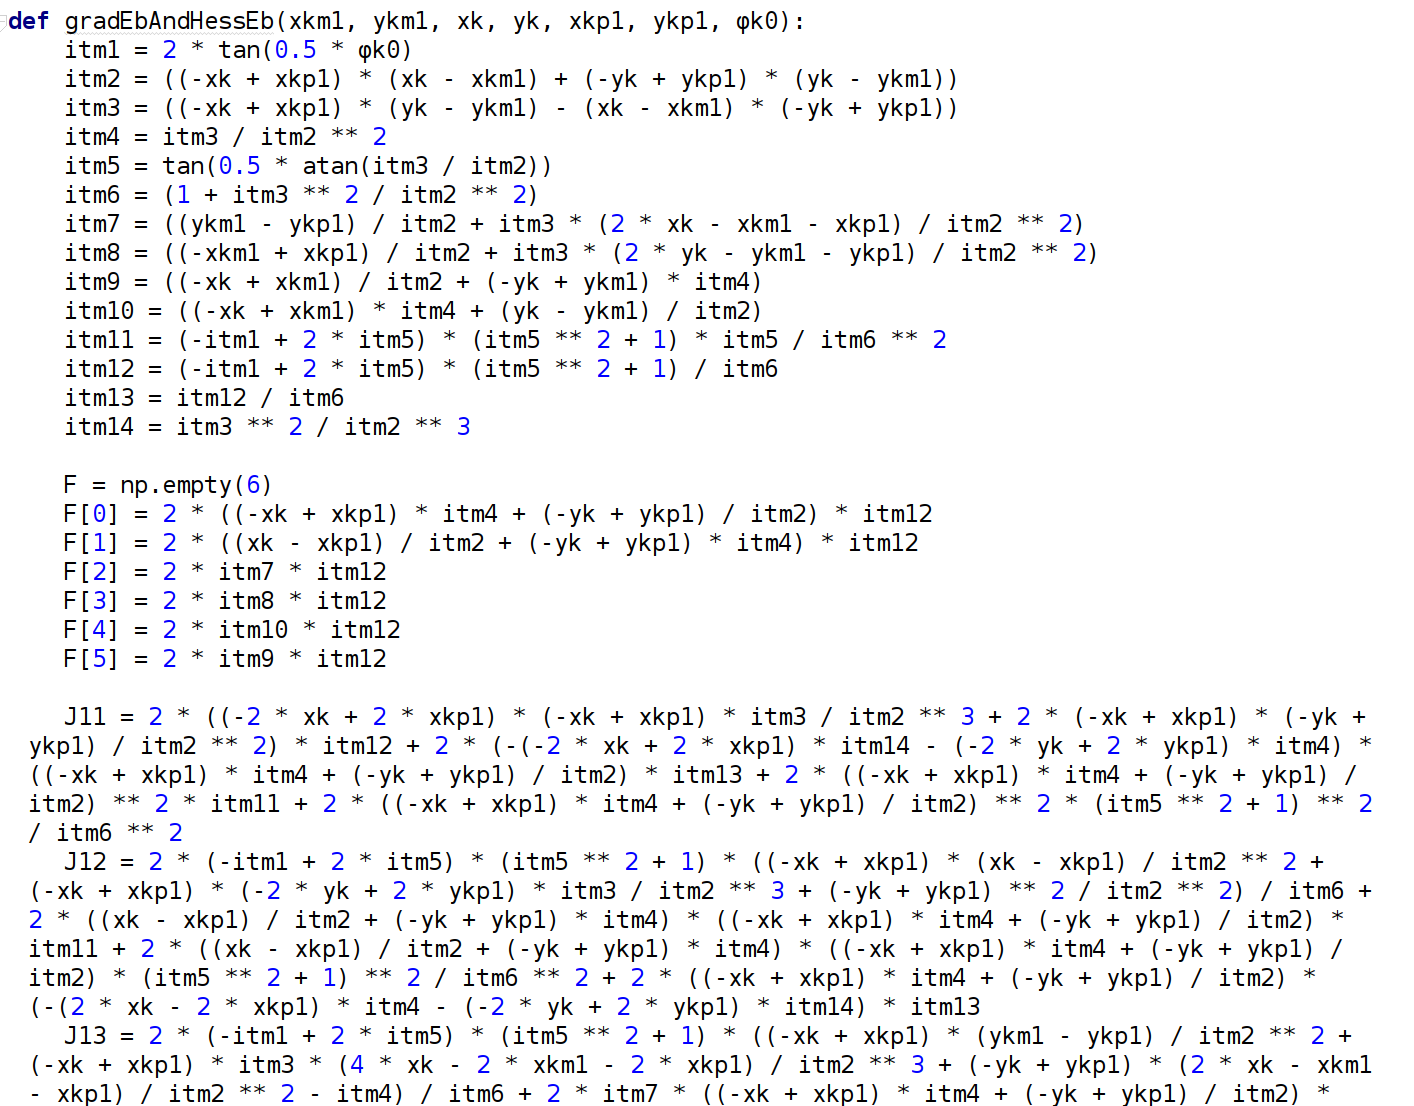
\includegraphics[width=0.9\textwidth]{res/getFb.png}
    	\begin{textblock}{0.3}[1,0](1,0.25)
		    \begin{center}
		    	\Large $30.6\,\mathrm s$\\$\Downarrow$\\$7.6\,\mathrm s$\\\bf $4\times$ faster
		    \end{center}
    	\end{textblock}
	\end{frame}
	\begin{frame}{What we did - Natural curvature}
		\begin{minipageparskip}{0.5\textwidth}
			When calculating bending energy, replace $\frac12EI(\phi_i)^2$ with $\frac12EI(\phi_i - \phi_{k0})^2$.
			
			The formulas for calculating $F$ and $J$ need to be changed (do differentiation again).
			
			\footnotesize
			To verify the result:
			\begin{itemize}
				\item Expect same result as previous code when $\phi_0$ = 0;
				\item Expect a straight beam to recover natural curvature when no external force applied.
			\end{itemize}
		\end{minipageparskip}%
		\hspace{0.05\textwidth}%
		\begin{minipageparskip}{0.45\textwidth}
			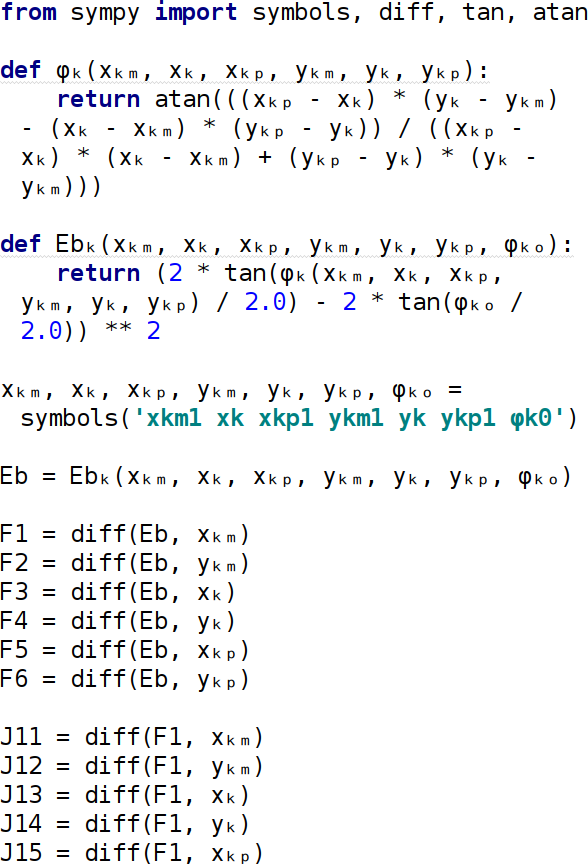
\includegraphics[width=\textwidth]{res/diff.png}
		\end{minipageparskip}
	\end{frame}
	\begin{frame}{What we did - Circular structure}
		\small
		Instead of $nv - 1$ edges, we have $nv$ edges.\\
		For bending, instead of $nv - 2$ components, we have $nv$ components.\\
		For stretching, instead of $nv - 1$ components, we have $nv$ components.
		
		When assembling the Jacobians, new components added to connect two ends together:
		
		\begin{center}
			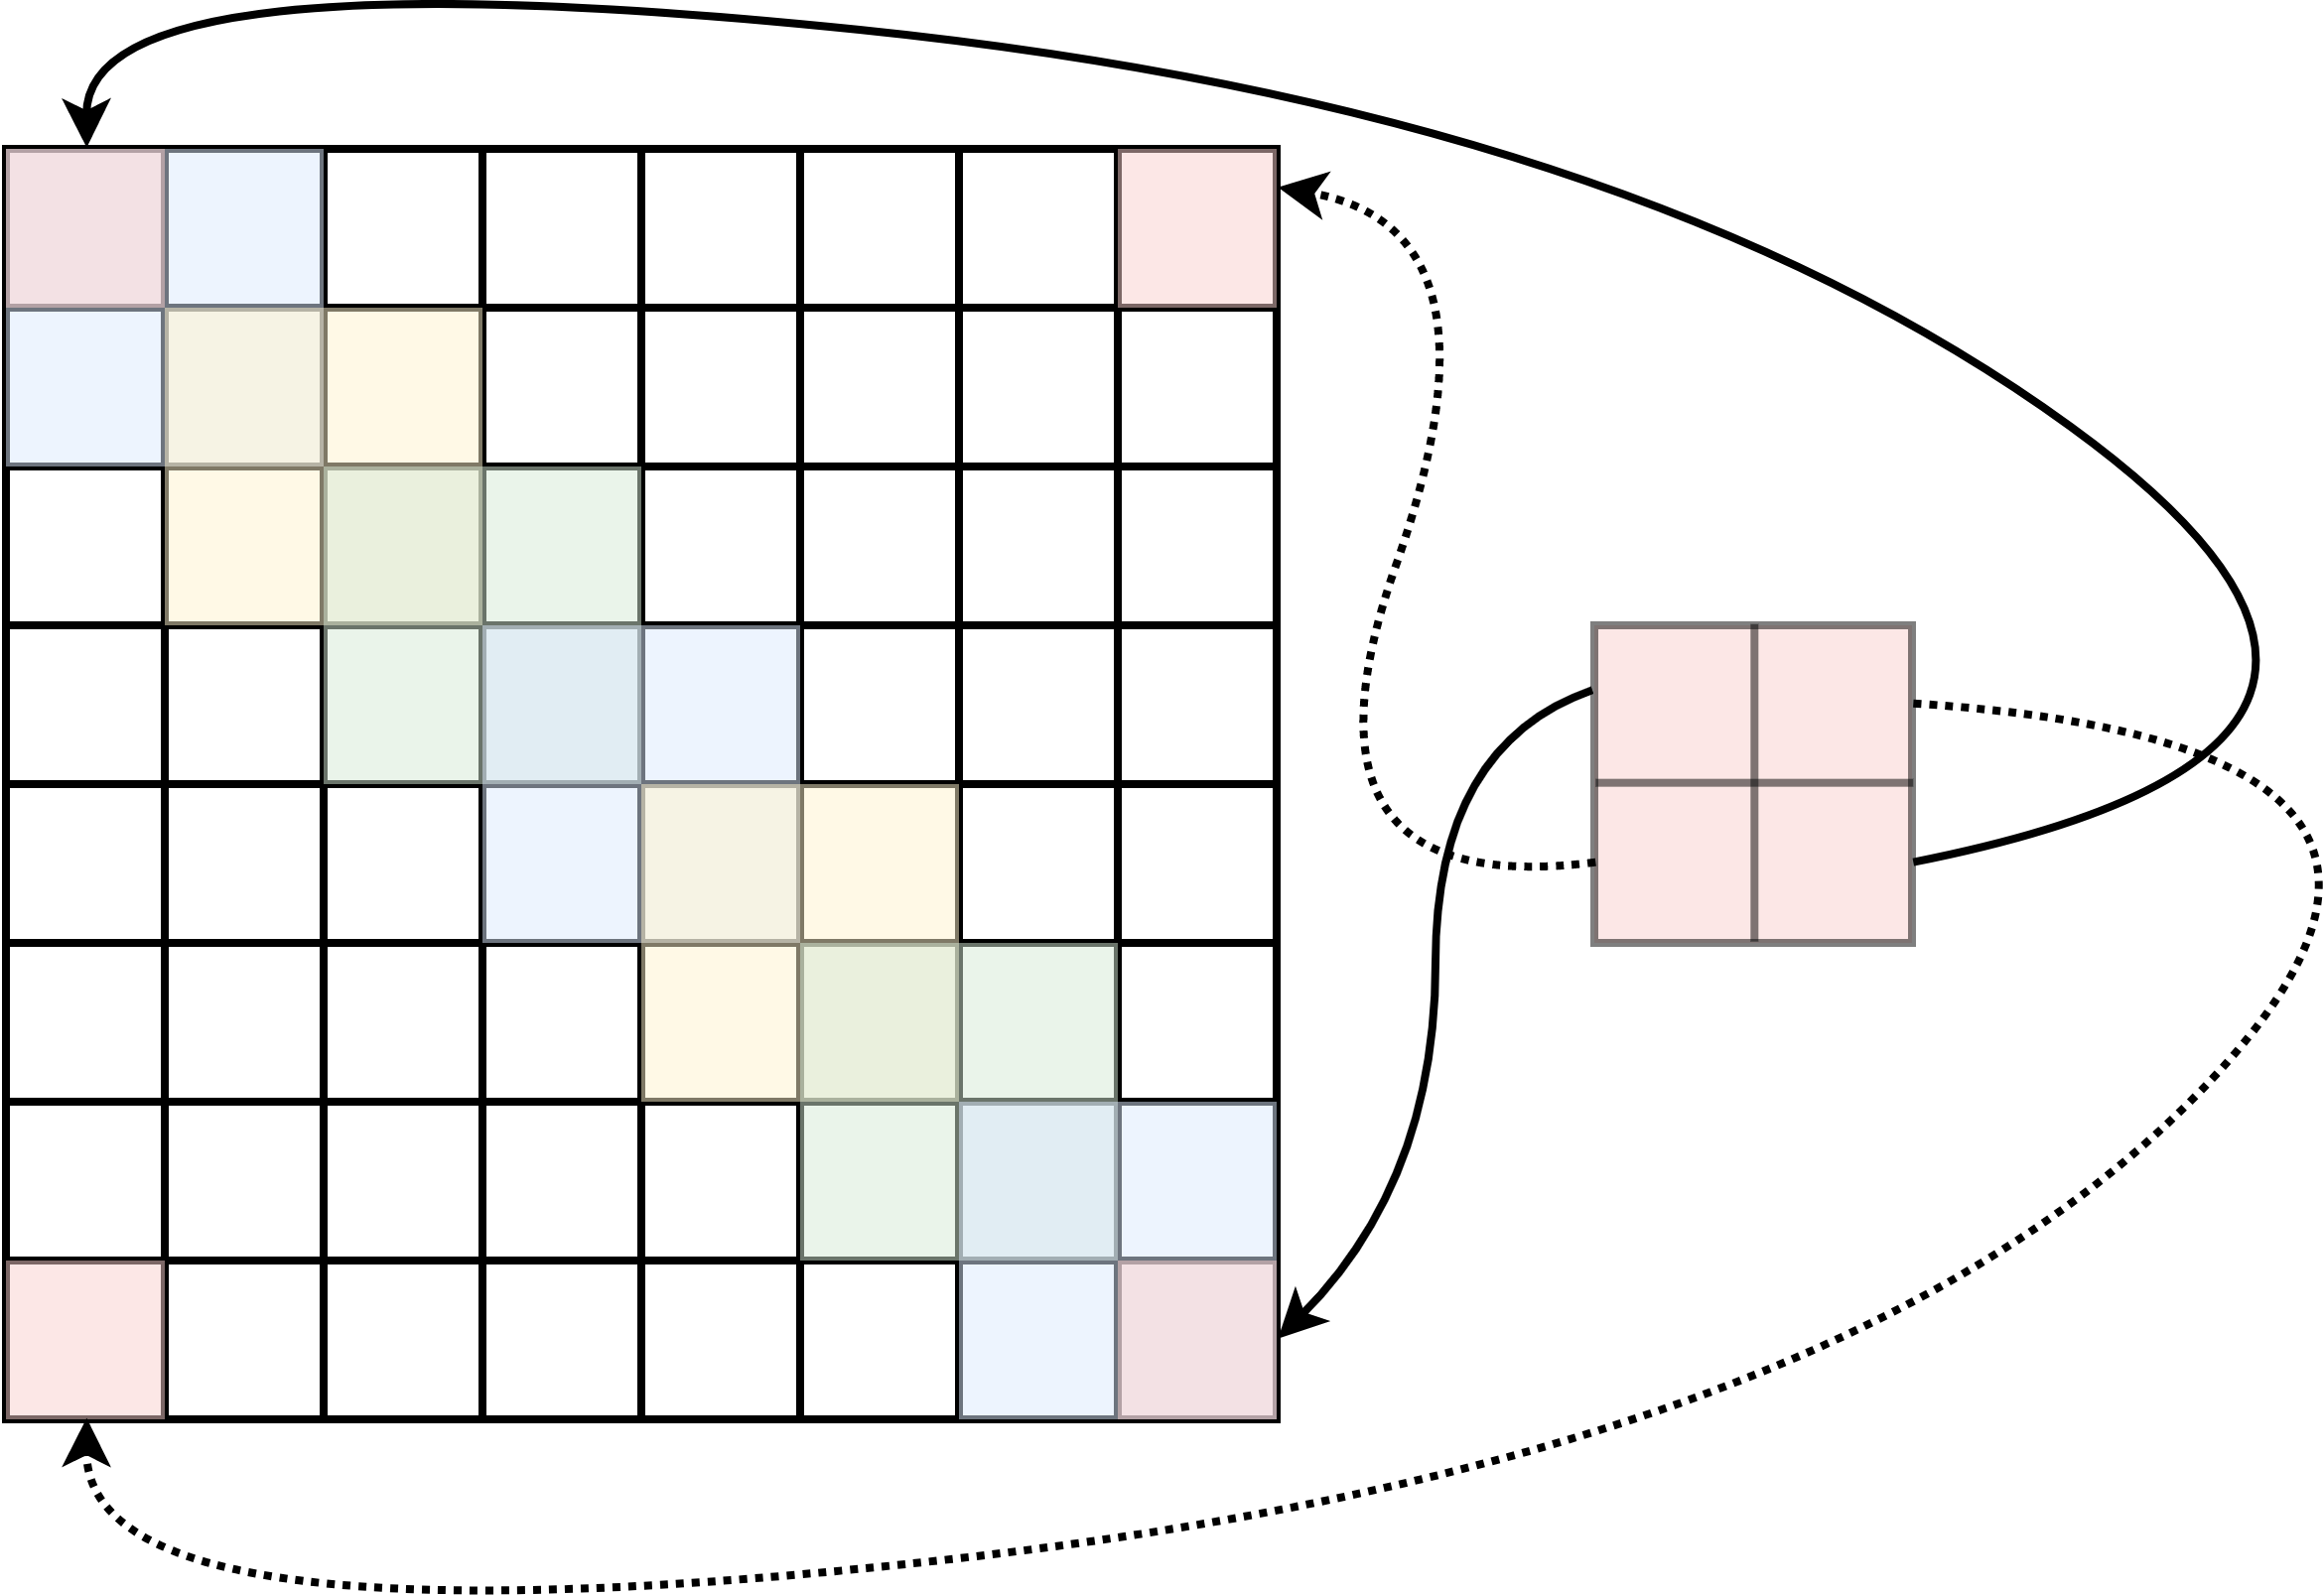
\includegraphics[width=0.6\textwidth]{res/composition.png}
		\end{center}
	\end{frame}
	\begin{frame}{What we did - Circular structure}
		Verify our code by running the ``hanging circle'':
		\vspace{0.5cm}
		\begin{widecenter}
			\begin{tabular}{ccc}
				$Y = 10^6\,\mathrm{Pa}$ & $Y = 10^7\,\mathrm{Pa}$ & $Y = 10^8\,\mathrm{Pa}$ \\
				\resvideo{1e6}{3.732}{3.708} & 
				\resvideo{1e7}{3.732}{3.708} & 
				\resvideo{1e8}{3.732}{3.708}
			\end{tabular}
		\end{widecenter}
	\end{frame}
	\begin{frame}{What we did - Inflation pressure}
		\begin{widecenter}
			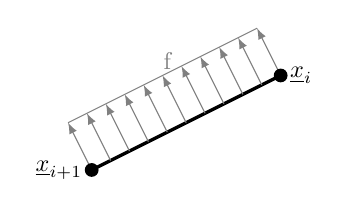
\begin{tikzpicture}[scale=0.6, every node/.style={scale=0.875}]
				\draw [very thick] (0,0) node [right] {$\underline x_i$} -- (-4,-2) node [left] {$\underline x_{i+1}$};
				\foreach \x in {0,...,10}
				\draw[gray,-latex,thin] (\x / 2.5 - 4,\x / 5 - 2) -- (\x / 2.5 - 4 - 0.5,\x / 5 - 2 + 1);
				\draw [gray,thin] (0 / 2.5 - 4 - 0.5,0 / 5 - 2 + 1) -- (10 / 2.5 - 4 - 0.5,10 / 5 - 2 + 1);
				\node [gray] at (5.5 / 2.5 - 4 - 0.6,5.5 / 5 - 2 + 1.2) {f};
				\node [circle,fill,minimum size=2mm,inner sep=0pt] at (0,0) {};
				\node [circle,fill,minimum size=2mm,inner sep=0pt] at (-4,-2) {};
			\end{tikzpicture}
			\hspace{0.1cm}
			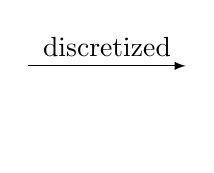
\begin{tikzpicture}[baseline=-1cm]
				\draw [-latex] (0,0) -- (2,0);
				\node [above] at (1,0) {discretized};
			\end{tikzpicture}
			\hspace{0.1cm}
			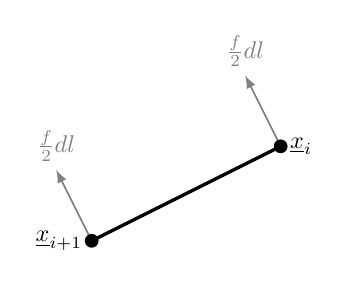
\begin{tikzpicture}[scale=0.6, every node/.style={scale=0.875}]
				\draw [very thick] (0,0) node [right] {$\underline x_i$} -- (-4,-2) node [left] {$\underline x_{i+1}$};
				\draw [gray,-latex,semithick] (0 / 2.5 - 4,0 / 5 - 2) -- (0 / 2.5 - 4 - 0.75,0 / 5 - 2 + 1.5) node [above] {$\frac{f}2 dl$};
				\draw [gray,-latex,semithick] (10 / 2.5 - 4,10 / 5 - 2) -- (10 / 2.5 - 4 - 0.75,10 / 5 - 2 + 1.5) node [above] {$\frac{f}2 dl$};
				\node [circle,fill,minimum size=2mm,inner sep=0pt] at (0,0) {};
				\node [circle,fill,minimum size=2mm,inner sep=0pt] at (-4,-2) {};
			\end{tikzpicture}
		\end{widecenter}
	
		With $\underline x_i$ and $\underline x_{i+1}$, we can easily calculate force exerted on those two points. 
		
		As force is dependent on actual positions of nodes, we need to add the variation into the Jabobian matrix. We simply take derivatives on the forces.
	\end{frame}
	\begin{frame}{What we did - Surface contact} 
		\textbf{Predictor-corrector method} is used.
		
		\footnotesize
		Assume a surface at $y = 0$, When doing time-marching, on each time step	:
		\begin{enumerate}
			\item Compute $\underline q(t)$ as before;
			\item Check if there exists any node whose $y < 0$. If there is any, set it as a temporarily constrained DOF with $y = 0$, and recompute current frame;
			\item Check if there exists any temporarily constrained DOF, such that the normal \textit{force} between the surface and the node is negative. Remove such temporary constraint, and recompute current frame.
		\end{enumerate}
		\begin{center}
			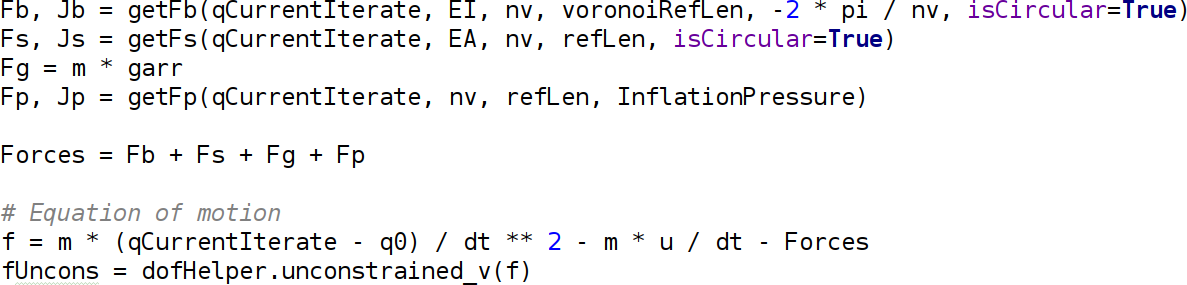
\includegraphics[width=\textwidth]{res/force.png}
		\end{center}
	\end{frame}
	\begin{frame}{What we did - Surface contact}
		In each frame:
		
		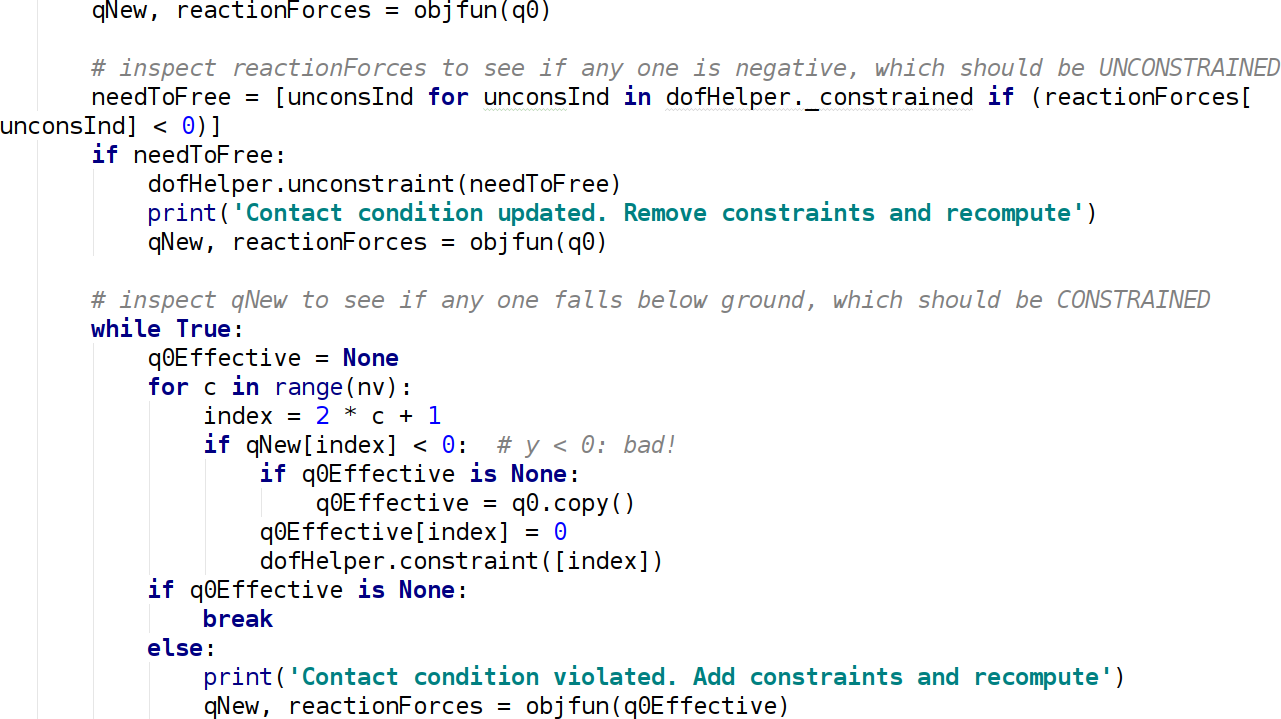
\includegraphics[width=1\textwidth]{res/corrector.png}
	\end{frame}
	\begin{frame}{Objective completed!}
		\begin{widecenter}
			\begin{tabular}{cc}
				Low pressure & High pressure \\
				\resvideo{l-pressure}{5.76875}{5.83125} & 
				\resvideo{h-pressure}{5.76875}{5.83125}
			\end{tabular}
		\end{widecenter}
	\end{frame}
	\begin{frame}{What we did - Damping}
		Without damping, we have oscillations.
		
		Naïve damping $\underline F_{d,i} \propto -\underline u_i$ ruins bulk motion (as our bulk velocity is high)
		
		So we use velocity relative to center of mass: $\underline F_{d,i} \propto -(\underline u_i - \underline u_{cm})$
		\vspace{0.5cm}
		\begin{widecenter}
			\begin{tabular}{ccc}
				No damping & Naïve damping & CM-Relative damping \\
				\resvideo{no-damp}{3.8467}{3.11} & 
				\resvideo{bad-damp}{3.6467}{3.11} & 
				\resvideo{good-damp}{3.8467}{3.11}
			\end{tabular}	
		\end{widecenter}
	\end{frame}
	\begin{frame}{Problem: Shape Jitter}
		\begin{widecenter}
			\resvideo{jitter}{4.3971}{3.75}
			\resvideo{jitter-slow}{5.8929}{3.75}
		\end{widecenter}
		\begin{itemize}
			\item Step size too large, everything bashed to ground before reacting
			\item Self-intersection occurs
		\end{itemize}
	\end{frame}
	\begin{frame}{Problem: Shape Jitter - Observations}
		\small
		Damping does not really help.
		
		Reducing time-step size helps. For the previous setup:
		
		\begin{widecenter}
			\begin{tabular}{cc}
				$dt = 4\times10^{-4}\,\mathrm s$ & $dt = 2.5\times10^{-4}\,\mathrm s$  \\
				\resvideo{4e-4}{4.59}{4.635} & 
				\resvideo{2.5e-4}{4.59}{4.59}
			\end{tabular}	
		\end{widecenter}
		
		Compared to initial time step size $5\times10^{-3}\,\mathrm s$. This takes $20\times$ more computational time! Almost unacceptable.
	\end{frame}
	\begin{frame}{Adaptive Time Stepping}
		``Adaptive Time Stepping'' in the assigned reading gave us some inspiration.
		
		When the time step is found too large by some criteria, we reduce the step size and try again. 
		
		When the adverse conditions are gone, step size is increased again.
		
		\begin{center}
			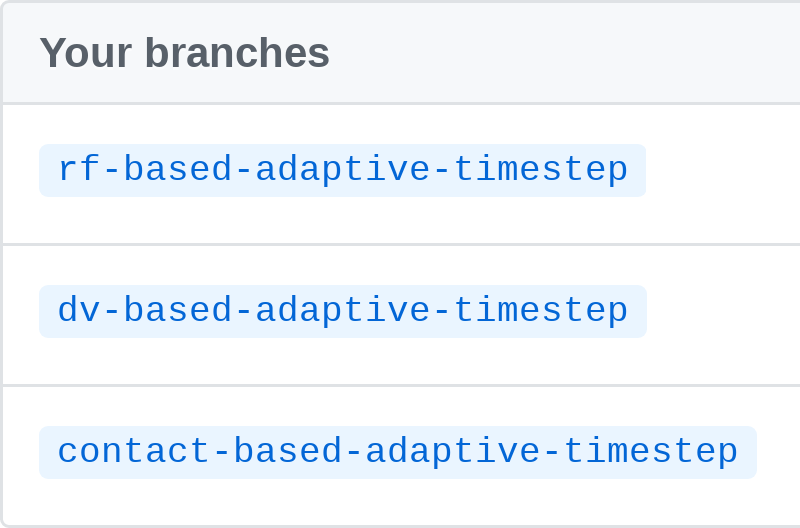
\includegraphics[width=0.4\textwidth]{res/branches.png}
		\end{center}
	\end{frame}
	\begin{frame}{Adaptive Time Stepping}
		\textbf{$\Delta v$-based adaptive time stepping}
		
		They use a $\Delta x$ threshold as criteria for deciding time steps. As our bulk velocity is high, we use the $\Delta v$ threshold instead.
		
		\textit{Not very effective:} Only saves $20\%$ steps. The oscillation also gives rapidly changing local velocity, we cannot distinguish the ``bashing''. 
		
		\textbf{Contact-based adaptive time stepping}
		
		Use small step when in contact with the surface. Otherwise use large step.
		
		\textit{Not very effective:} Not flexible enough (only two step sizes); step size is small even when resting on the surface.
	\end{frame}
	\begin{frame}{Adaptive Time Stepping}
		\begin{minipageparskip}{0.45\textwidth}
			\small
			\textbf{Reaction force-based adaptive time stepping}
			
			Step size should be inverse proportional to the maximum nodal reaction force from the ground.\\
			We use $F_{max}dt \leq 0.008\,\mathrm{N\cdot s}$ as the threshold for previous setup.
		
			Instead of ``decreasing by half, increasing by doubling'' (as used in the paper), we examine $\frac{F_{max}dt}{0.008\,\mathrm{N\cdot s}}$ to decide how much we should increase/decrease.
		\end{minipageparskip}%
		\begin{minipageparskip}{0.55\textwidth}
			\tiny
			\hfill
			\begin{tikzpicture}
				\begin{axis}[width=6cm,height=4cm,xlabel={$t$ [$\mathrm s$]},ylabel={$F_{max}$ [$\mathrm N$]},xmax=0.1,xticklabel style={/pgf/number format/fixed}]
					\addplot[black] table [x=t, y=f, col sep=comma, mark=none] {res/f-vs-dt.csv};
				\end{axis}
			\end{tikzpicture}
			
			\hfill
			\begin{tikzpicture}
				\begin{axis}[width=6cm,height=4cm,xlabel={$t$ [$\mathrm s$]},ylabel={$dt$ [$\mathrm s$]},xmax=0.1,xticklabel style={/pgf/number format/fixed}]
					\addplot[black] table [x=t, y=dt, col sep=comma, mark=none] {res/f-vs-dt.csv};
				\end{axis}
			\end{tikzpicture}
		\end{minipageparskip}
	\end{frame}
	\begin{frame}{Adaptive Time Stepping}
		For a $2\,\mathrm s$ simulation, only $487$ steps attempted, resulting in $437$ valid steps. 
		
		Compared to $400$ steps (initial setup $dt = 5\times10^{-3}\,\mathrm s$), we only need $\sim20\%$ more steps, instead of $\sim2000\%$.
		
		\begin{widecenter}
			\resvideo{ats}{5.695}{4.635}
			\resvideo{ats-slow}{5.155}{4.635}
		\end{widecenter}
	\end{frame}
	\begin{frame}{Surface friction considered}
		For all nodes in contact with the surface, a friction force proportional to its velocity is applied: $F_{f,i} \propto - u_{i}$.
		
		\begin{widecenter}
			\resvideo{no-friction}{6.856875}{5.214375}
			\resvideo{friction-0.2}{5.175}{5.214375}
		\end{widecenter}
	\end{frame}
	\begin{frame}{More realistic friction}
		\begin{minipageparskip}{0.5\textwidth}
			\small
			Model local friction be proportional to the local normal force: $F_{f,i} = -\mathrm{sign}(u_{i}) \mu F_{N,i}$.
			
			However, normal force is acquired after solving EOM. We don't know it when forming EOM with $F_{f,i}$.
		\end{minipageparskip}%
		\begin{minipageparskip}{0.5\textwidth}
			\tiny
			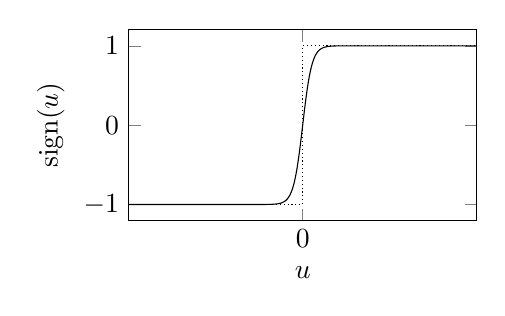
\begin{tikzpicture}
				\begin{axis}[width=6cm,height=4cm,xlabel={$u$},ylabel={$\mathrm{sign}(u)$},xmin=-7.5,xmax=7.5,xtick={0},domain=-7.5:7.5]
				\addplot[no marks, densely dotted] coordinates {(-7.5,-1) (0,-1) (0,1) (7.5,1)};
				\addplot[no marks, samples=600] {2 / (1 + exp(-5 * x)) - 1};
				\end{axis}
			\end{tikzpicture}
		\end{minipageparskip}
	
		\small
		What if we use the normal force $F_{N}$ acquired in previous Newton-Raphson iteration?
		\begin{itemize}
			\item The result is still accurate when iteration converges.
			\item However, convergence is not guaranteed, because we don't have a reliable $J_f$.
		\end{itemize}
	\end{frame}
	\begin{frame}{More realistic friction}
		However, convergence is possible with an approximation, using $\mathrm{sign}(u_{t=t_{k-1}})$ instead of $\mathrm{sign}(u_{t=t_k})$.
		
		\begin{center}
			\resvideo{friction}{8.1}{5.562}
		\end{center}
	\end{frame}
	\begin{frame}{What's next}
		\begin{itemize}
			\item Better simulation of friction
			\item Self-intersection prevention
			\item Compare with results from literature
			\item 3-D sphere (with discrete shells)
		\end{itemize}
	\end{frame}
	\begin{frame}{Project on GitHub now!}
		All code, results (and these slides) uploaded to
		
		\begin{center}
			\url{https://github.com/kmxz/mae259b-project}
			
			\qrcode[height=2.75cm]{https://github.com/kmxz/mae259b-project}
		\end{center}
	\end{frame}
\end{document}